\documentclass[14pt,fleqn]{extarticle}
\RequirePackage{prepwell}
\previewoff
\begin{document}

\newcommand\yone{4-x^2} 
\newcommand\ytwo{4- \left(x-2 \right)^2}
\newcommand\intg{\frac{a^2}{2}\sin^{-1}\frac{x}{a}+x\cdot\sqrt{a^2-x^2}}

%text
Using integration, find the area of the region 
enclosed between the two circles 
\[ \quad x^2+y^2=4\text{ and } (x-2)^2 + y^2 = 4 \]
%

\newcard

A circle with center at $(a,b)$ and radius $R$ has the equation 
\[ \qquad \left(x-a \right)^2 + \left(y-b \right)^2 = R^2 \]

When one compares this with the equations of the given circles, one can see that 
\begin{center}
  \begin{tabular}{NNN}
   \toprule
        \text{Circle} & \text{Center} & \text{Radius}  \\
   \midrule 
   x^2 + y^2 = 4 & (0,0) & 2 \\
    \midrule 
    \left(x-2 \right)^2 + y^2 = 4 & (2,0) & 2 \\
    \bottomrule
  \end{tabular}
\end{center}
And hence, the two circles are as shown below -- with $A$ as the required area 

\begin{center}
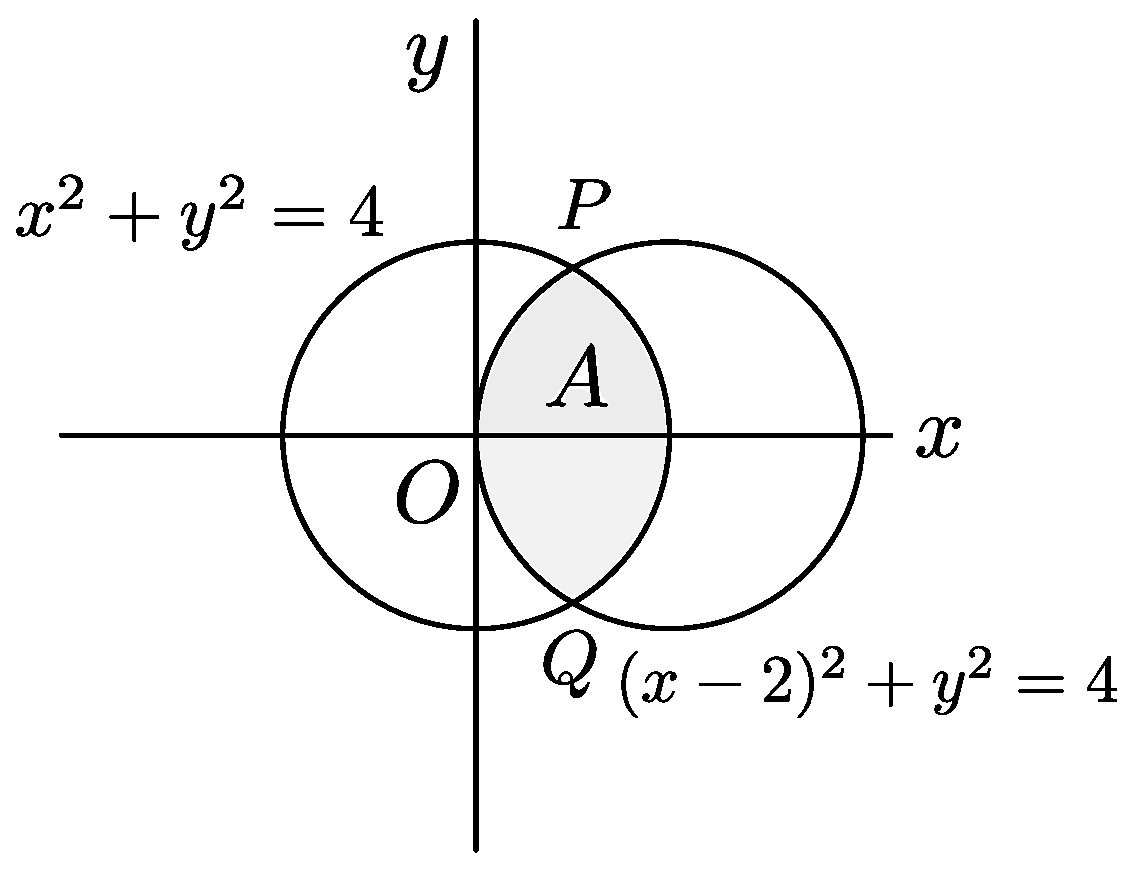
\includegraphics[scale=0.35]{figure.eps} 
\end{center} 

\newcard

The two circles intersect at 
\begin{align}
P &= \left(1,\sqrt{3} \right)\text{ and } Q = \left(1, -\sqrt{3} \right)
\end{align}

\newcard 

The two circles will intersect when 
\begin{align}
	y = \yone &= \ytwo \\
	\text{or } 4-x^2 &= 4 - \left(x^2- 4x + 4 \right) \\
	\implies \yone &= x^2 + 4x \text{ or } 2\cdot \left(x-1 \right)^2 = 0 \\
	\therefore x = 1&\text{ and } y = \sqrt{\yone} = \pm \sqrt{3} 
\end{align}

Hence, the \underline{two points} where the two circles will intersect are 
\[ \qquad P = \left(1,\sqrt{3} \right)\text{ and } Q = \left(1,-\sqrt{3} \right)\]

\newcard

\smallmath 
\begin{align}
A &= 2 \left[\int_0^1 \sqrt{\ytwo}\cdot dx + \int_1^2 \sqrt{\yone}\cdot dx  \right] \\
&= 4\int_1^2 \sqrt{\yone}\cdot dx 
\end{align}

\newcard

The required area $A$ is divided in half by the $x-$axis \newline 

It is further divided in half by the line $PQ$, thereby splitting $A$ into 
four equal parts -- $a,b,c$ and $d$ \newline 

\begin{center}
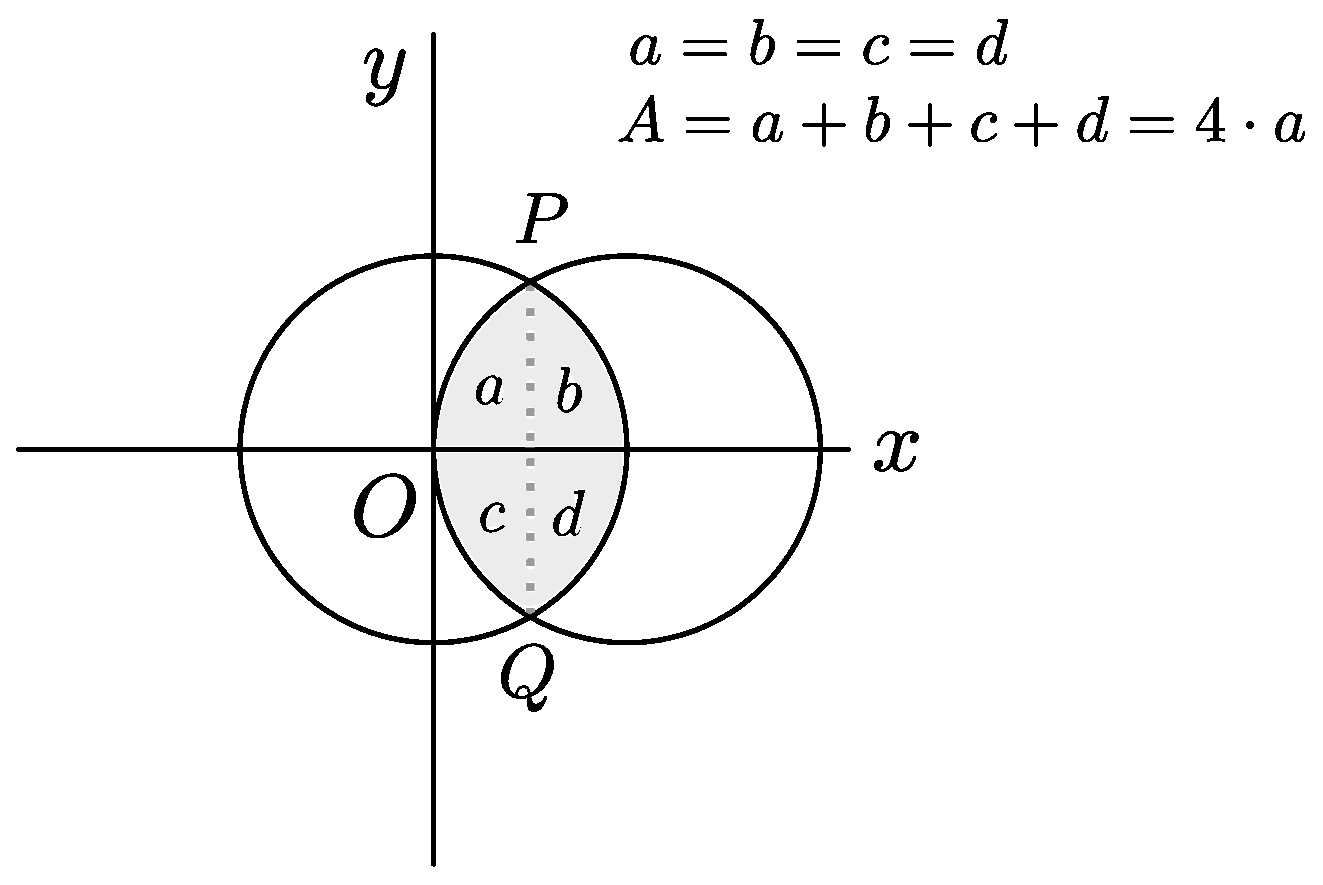
\includegraphics[scale=0.35]{fig-2.eps} 
\end{center} 

And therefore, we can see that 
\smallmath
\begin{align}
A &= 2\cdot \left(a+b \right) \\
&= 2 \left[\underbrace{\int_0^1 \sqrt{\ytwo}\cdot dx}_{a} + \underbrace{\int_1^2 \sqrt{\yone}\cdot dx}_{b} \right] \\
&= 4 \underbrace{\int_1^2 \sqrt{\yone}\cdot dx}_{b} \text{ (easier to evaluate)}
\end{align}

\newcard 

\[ A = \frac{4}{3}\cdot \left(2\pi-3\sqrt{3} \right)\]

\newcard 

\[ A = \frac{4}{3}\cdot \left(\pi-\sqrt{3} \right)\]

\newcard 
\begin{align}
A &= 4 \left[\int_1^2 \sqrt{\yone}\cdot dx \right] \\
&= 4\cdot \underbrace{\left[2\sin^{-1}\frac{x}{2} + x\sqrt{\yone} \right]_1^2}_{\intg} \\
&= 4 \left[\left(2 \cdot\frac{\pi}{2} + 0 \right) - \left(2\cdot\frac{\pi}{6} + \sqrt{3} \right) \right] \\
&= \frac{8\pi}{3} - 4\sqrt{3} = \frac{4}{3}\cdot \left(2\pi-3\sqrt{3} \right)
\end{align}
\end{document}